% Chapter Template

\chapter{Empirical Study} % Main chapter title

\label{ChapterX} % Change X to a consecutive number; for referencing this chapter elsewhere, use \ref{ChapterX}

%----------------------------------------------------------------------------------------
%	SECTION 1
%----------------------------------------------------------------------------------------
\section{Study Design}

The main \textit{goal} of this study is to validate whether the proposed pipeline is feasible, when using a software engineering task as reference and when applied directly to APK files. The \textit{perspective} of the study is of researchers interested in enabling comprehensive solutions for the needed improvement of android app development process. Regarding the \textit{context}, it consist of 54 open source Android applications. In particular, this study aims at answering the following research questions:

\begin{itemize}
	\item \textit{\textbf{$RQ_{1}$}: What is the impact of generating mutants at APK level ?}
	\begin{itemize}
		\item \textit{\textbf{$RQ_{1.1}$}:What is the impact in terms of the amount of generated mutants?}
		\item \textit{\textbf{$RQ_{1.2}$}:What is the impact in terms of the time required to generate a mutant?}
		\item \textit{\textbf{$RQ_{1.3}$}:What is the impact in terms of the amount of compiled mutants?}
		\item \textit{\textbf{$RQ_{1.4}$}:What is the impact in terms of the time required to compile a mutant?}
	\end{itemize}
\end{itemize}

\section{Context of the Study}

In order to present a fair comparison between MutAPK and MDroid+, we have used the same apps MDroid+ used for their experiments. This 54 applications presented in Table \ref{tab:alufs} belong to 16 different categories of the Google Play Store. It is worth noticing that these 54 applications are open source and allows us to study the way code statements are translated from JAVA to SMALI.

In order to collect data that allow us to answer the research question, we compared MutAPK to an existing tool for mutation testing that works at source code level ( MDroid+ \cite{linares2017enabling} ). 
The experiments were executed on a class-server machine. 
Note that in MutAPK, we implemented only 35 of 38 operators listed in Table \ref{tab:cmol} because the other 3 operators lead to non-compilable results. In order to analyze the impact of mutant generation process in MutAPK, we collect: (i) number of mutants generated per mutation operator per application; (ii) number of mutants that compile after mutation; (iii) mutant generation time (\textit{i.e.,} the time required to generate each mutant) and (iv) mutant building times (\textit{i.e.,} the time required to compile each APK file)
\begin{table}[t]
	\centering
	\caption{Applications used for the study}
	\label{tab:alufs}
	\resizebox{0.80\textwidth}{!}{\begin{tabular}{clllc}
			App ID & App Name & Category & Package Name & Version \\
			\hline\hline \\
			1 & A2DP Volume & Transportation & a2dp.Vol & 2.8.11 \\
			2 & AardDictionary & Books \& Reference & aarddict.android & 1.4.1 \\
			3 & FTP Server & Tools & be.ppareit.swiftp\_free & 2.2 \\
			4 & Bites & Lifestyle & caldwell.ben.bites & 1.3 \\
			5 & Battery Circle & Tools & ch.blinkenlights.battery & 1.81 \\
			6 & KeePassDroid & Tools & com.android.keepass & 1.9.8 \\
			7 & LolcatBuilder & Entertainment & com.android.lolcat & 2 \\
			8 & SpriteMethodTest & Sample & com.android.spritemethodtest & 1 \\
			9 & Alarm Clock & Tools & com.angrydoughnuts.android.alarmclock & 1.7 \\
			10 & Translate & Tools & com.beust.android.translate & 1.6 \\
			11 & Quick Settings & Tools & com.bwx.bequick & 1.9.9.4 \\
			12 & Manpages & Productivity & com.chmod0.manpages & 1.51 \\
			13 & BookCatalogue & Productivity & com.eleybourn.bookcatalogue & 3.8 \\
			14 & Mileage & Finance & com.evancharlton.mileage & 3.1.1 \\
			15 & Auto Answer & Tools & com.everysoft.autoanswer & 1.5 \\
			16 & Amazed & Casual & com.example.amazed & 2.0.2 \\
			17 & RandomMusicPlayer & Music & com.example.android.musicplayer & 1 \\
			18 & AnyCut & Productivity & com.example.anycut & 0.5 \\
			19 & HNDroid & News \& Magazines & com.gluegadget.hndroid & 0.2.1 \\
			20 & SpriteText & Sample & com.google.android.opengles.spritetext & - \\
			21 & Triangle & Sample & com.google.android.opengles.triangle & - \\
			22 & Photostream & Media \& Video & com.google.android.photostream & 1.1 \\
			23 & Multi SMS & Communication & com.hectorone.multismssender & 2.3 \\
			24 & World Clock & Tools & com.irahul.worldclock & 0.6 \\
			25 & SyncMyPix & Media \& Video & com.nloko.android.syncmypix & 0.15 \\
			26 & Jamendo & Music & com.teleca.jamendo & 1.0.6-legacy \\
			27 & Yahtzee & Casual & com.tum.yahtzee & 1 \\
			28 & Sanity & Communication & cri.sanity & 2.11 \\
			29 & Mirrored & News \& Magazines & de.homac.Mirrored & 0.2.3 \\
			30 & FileExplorer & Productivity & edu.killerud.fileexplorer & 1 \\
			31 & WeightChart & Health \& Fitness & es.senselesssolutions.gpl.weightchart &	 1.0.4 \\
			32 & SoundBoard & Sample & hiof.enigma.android.soundboard & 1 \\
			33 & ADSdroid & Books \& Reference & hu.vsza.adsdroid & 1.2 \\
			34 & myLock & Tools & i4nc4mp.myLock & 42 \\
			35 & LockPatternGenerator & Tools & in.shick.lockpatterngenerator & 2 \\
			36 & MunchLife & Entertainment & info.bpace.munchlife & 1.4.2 \\
			37 & aGrep & Tools & jp.sblo.pandora.aGrep & 0.2.1 \\
			38 & CountdownTimer & Tools & net.everythingandroid.timer & 1.1.0 \\
			39 & LearnMusicNotes & Puzzle & net.fercanet.LNM & 1.2 \\
			40 & NetCounter & Tools & net.jaqpot.netcounter & 0.14.1 \\
			41 & TippyTipper & Finance & net.mandaria.tippytipper & 1.1.3 \\
			42 & BaterryDog & Tools & net.sf.andbatdog.batterydog & 0.1.1 \\
			43 & Bomber & Casual & org.beide.bomber & 1 \\
			44 & Dialer2 & Productivity & org.dnaq.dialer2 & 2.9 \\
			45 & FrozenBubble & Puzzle & org.jfedor.frozenbubble & 1.12 \\
			46 & aLogCat & Tools & org.jtb.alogcat & 2.6.1 \\
			47 & AnyMemo\_135 & Education & org.liberty.android.fantastischmemo & 8.3.1 \\
			48 & PasswordMakerPro & Tools & org.passwordmaker.android & 1.1.7 \\
			49 & Blokish & Puzzle & org.scoutant.blokish & 2 \\
			50 & ZooBorns & Entertainment & org.smerty.zooborns & 1.4.4 \\
			51 & Wordpress\_394 & Productivity & org.tomdroid & 0.5.0 \\
			52 & MyExpenses & Finance & org.totschnig.myexpenses & 1.6.0 \\
			53 & ImportContacts & Tools & org.waxworlds.edam.importcontacts & 1.1 \\
			54 & Wikipedia & Books \& Reference & org.wikipedia & 1.2.1 \\
		\end{tabular}
	}
\end{table}

\section{Results: Impact of generating mutants at APK level}

\begin{table}[t]
	\centering
	\caption{Comparision at Mutation Operator Level}
	\label{tab:cmol}
	\resizebox{\textwidth}{!}{\begin{tabular}{lC{2cm}lrrrrrrrr}
			&&                      & \multicolumn{2}{c}{\begin{tabular}[c]{@{}c@{}}Amount Mutants\\ Generated\end{tabular}} & \multicolumn{2}{c}{\begin{tabular}[c]{@{}c@{}}Amount Mutants\\ Compiled\end{tabular}}\\
			ID&Mutation Type&Operator Name& MutAPK                                  & MDroid+                                  & MutAPK                                  & MDroid+                                 \\
			\hline \hline \\
			1&Text&ActivityNotDefined&385&384&385&383\\
			2&AST&DifferentActivityIntentDefinition&482&358&120&356\\
			3&Text&InvalidActivityName&383&382&383&382\\
			4&AST&InvalidKeyIntentPutExtra&477&459&62&456\\
			5&Text&InvalidLabel&214&214&214&214\\
			6&AST&NullIntent&482&559&413&556\\
			7&AST&NullValueIntentPutExtra&477&459&452&459\\
			8&Text&WrongMainActivity&56&56&56&56\\
			9&Text&MissingPermissionManifest&227&229&227&229\\
			10&Text&WrongStringResource&3432&3394&3430&3394\\
			11&AST&NotParcelable&0&7&0&1\\
			12&Text&SDKVersion&0&66&0&66\\
			13&AST&LengthyBackEndService&15&8&15&8\\
			14&AST&LongConnectionTimeOut&0&0&0&0\\
			15&AST&BluetoothAdapterAlwaysEnabled&0&4&0&4\\
			16&AST&NullBluetoothAdapter&9&9&9&9\\
			17&AST&InvalidURI&2&2&1&2\\
			18&AST&NullGPSLocation&2&1&2&1\\
			19&AST&InvalidDate&20&40&20&40\\
			20&AST&NullBackEndServiceReturn&34&8&25&7\\
			21&AST&InvalidMethodCallArgument&0&0&0&0\\
			22&AST&NullMethodCallArgument&63441&0&63437&0\\
			23&AST&ClosingNullCursor&222&179&221&166\\
			24&AST&InvalidIndexQueryParameter&82&7&82&6\\
			25&AST&InvalidSQLQuery&82&33&82&33\\
			26&AST&ViewComponentNotVisible&398&347&396&342\\
			27&AST&FindViewByIdReturnsNull&915&413&803&413\\
			28&Text&InvalidColor&47&52&44&52\\
			29&AST&InvalidViewFocus&397&0&393&0\\
			30&AST&BuggyGUIListener&0&122&0&122\\
			31&AST&InvalidIDFindView&915&456&0&452\\
			32&AST&   InvalidFilePath&228&220&226&220\\
			33&AST&NullInputStream&90&61&88&61\\
			34&AST&NotSerializable&0&15&0&8\\
			35&AST&OOMLargeImage&7&7&7&3\\
			36&AST&LengthyGUIListener&339&122&335&122\\
			37&AST&NullOutputStream&59&45&59&45\\
			38&AST&LengthyGUICreation&336&129&330&129\\
			\hline \hline\\
			\multicolumn{3}{c}{\begin{tabular}[c]{@{}c@{}}Total\end{tabular}}&74255&8847&72317&8797\\
	\end{tabular}}
\end{table}

\textbf{\textit{$RQ_{1.1}$}}: To study our results, we present them in two stages, first we show a comparison where only the 33 mutants  in both MDroid+ and MutAPK are taken into account. In Figure \ref{fig:s22agmbp} we show the total amount of generated mutants per app. MutAPK generates around 30 more mutants per app (17\% more than MDroid+). However, if all operators are taken into account, the difference between the amount of mutants get bigger. Figure \ref{fig:agmbp} shows the amount of generated mutants per app. As it can be seen, MutAPK outperforms MDroid+ generating in average 1211 more mutants per app, this corresponds to 7.3 times more mutants. For further analysis of the results at app level, we added the Tables \ref{tab:cal1} and \ref{tab:cal2}, where all info collected is summarized around apps (See Appendix A). Also, we show in Figure \ref{fig:s22agmmobp} that the amount of mutants generated per mutant operator are very similar between MutAPK and MDroid+. It is worth nothing that this figure does not take into account the 63441 mutants generated by one of the operators implemented only in MutAPK. 

\textbf{\textit{$RQ_{1.2}$}}: If we consider again only the 33 shared mutants, in Figure \ref{fig:s22pncmbp} we can see that MutAPK generates around 16\% of non-compilable mutants while MDroid+ generates only 0.5\%. Nevertheless, when using all operators MutAPK generates around 2.36\% of non-compilable mutants while MDroid+ lightly increase its rate to 0.6\%. At the same time, Figure \ref{fig:s22pncmmobp} shows the percentage of non-compilable mutants in terms of the mutant operators, from this we can see that there is also a similar behavior for both. Specifically, MutAPK generates in average 0.1\% non-compilable mutants while MDroid generates 0.05\%.

\textbf{\textit{$RQ_{1.3}$}}: The most important result is the execution time. MutAPK takes only 3\% of the time ( 144,66ms ) required by MDroid+ ( 4,6 seconds) to mutate a copy of the app. Therefore, due to the infraestructure used to run our study, MutAPK takes 9 seconds to generate all mutants for an app (on average), while MDroid takes 19 seconds. 

\textbf{\textit{$RQ_{1.4}$}}: For compilation, MutAPK spends only 6.3\% of the time required by MDroid+ to compile a mutant. Consequently, MutAPK takes 11 min to compile all mutants for an app (on average) while MDroid+ takes 13 min.


Finally, if all mutant operators are selected, MutAPK takes around 9.63 hours to complete the mutation and compilation process for the 54 apps while MDroid+ takes 12 hours.  It is worth remembering that MutAPK generates around 7.3 times more mutants than MDroid+. Therefore, the remaining time could be used by developers,  practitioners, and servers to other software engineering activities. Additionally, as MutAPK generates more mutants, the generated search/bugs space  might be more comprehensive, which means that the quality of the test suite can be tested in a more wide sense.

\begin{landscape}
	\centering
\begin{figure}[t]
	\centering
	\subfigure[\# of Mutants Generated per App without not shared operators]{
		\label{fig:s22agmbp}
		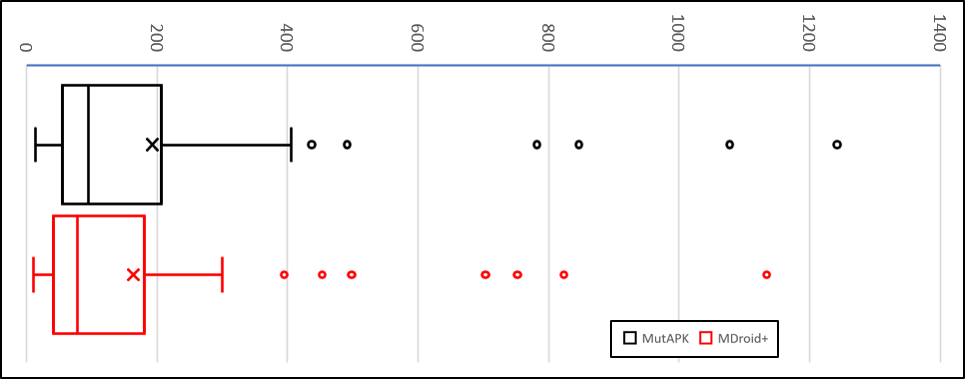
\includegraphics[width=0.35\textheight]{Figures/S22AmountGenMutBP}}
	\subfigure[\% Non-Compilable Mutants without not shared operators]{
		\label{fig:s22pncmbp}
		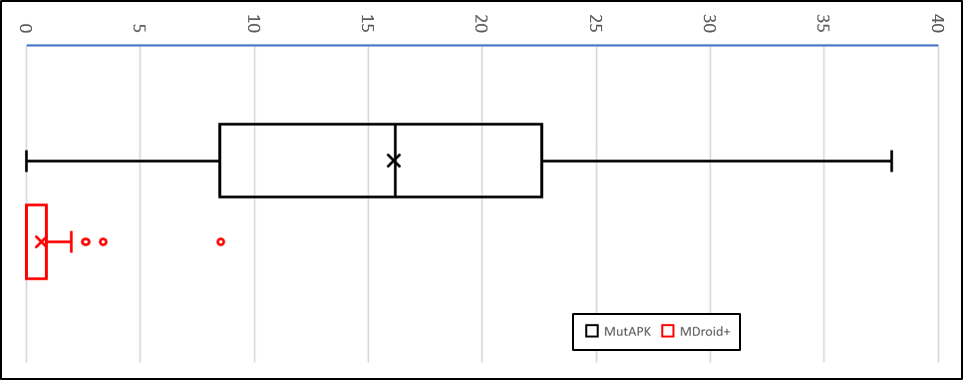
\includegraphics[width=0.35\textheight]{Figures/S22PercNonCompMutBP}}
	\subfigure[\# of Mutants Generated per App]{
		\label{fig:agmbp}
		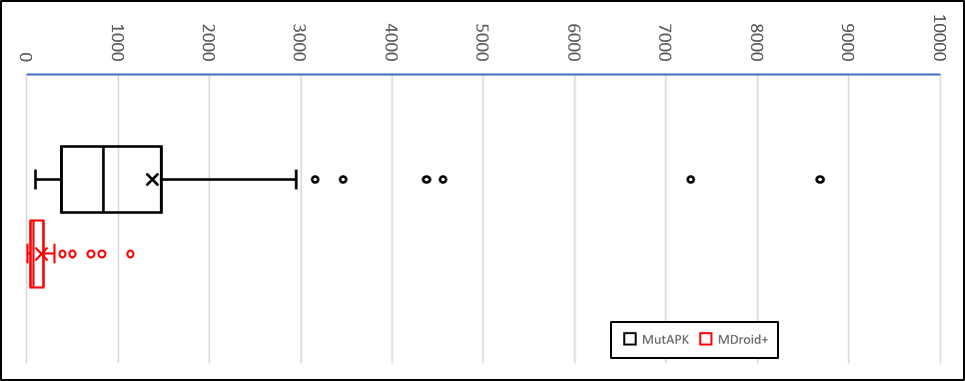
\includegraphics[width=0.35\textheight]{Figures/AmountGenMutBP}}
	\subfigure[\% Non-Compilable Mutants]{
		\label{fig:pncmbp}
		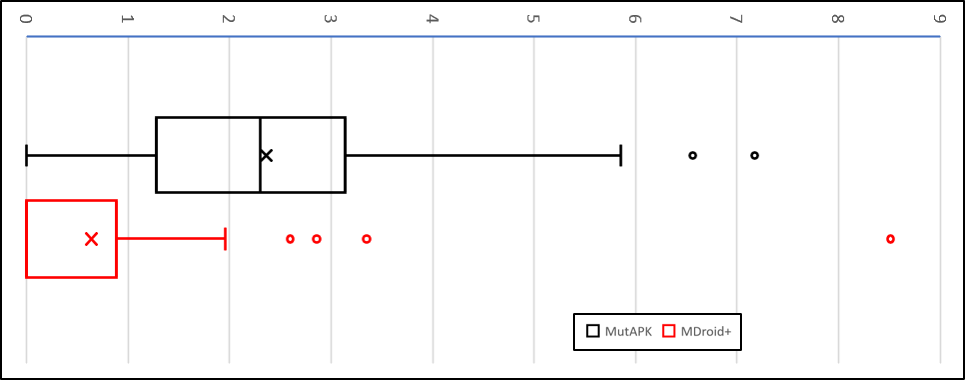
\includegraphics[width=0.35\textheight]{Figures/PercNonCompMutBP}}
	\subfigure[\# of Mutants Generated per mutant operator]{
		\label{fig:s22agmmobp}
		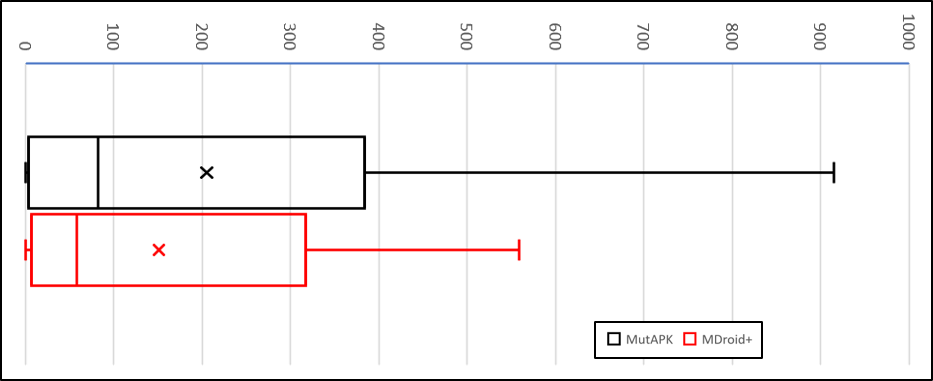
\includegraphics[width=0.35\textheight]{Figures/S22AmountGenMutMOBP}}
	\subfigure[\% Non-Compilable Mutants per mutant operator]{
		\label{fig:s22pncmmobp}
		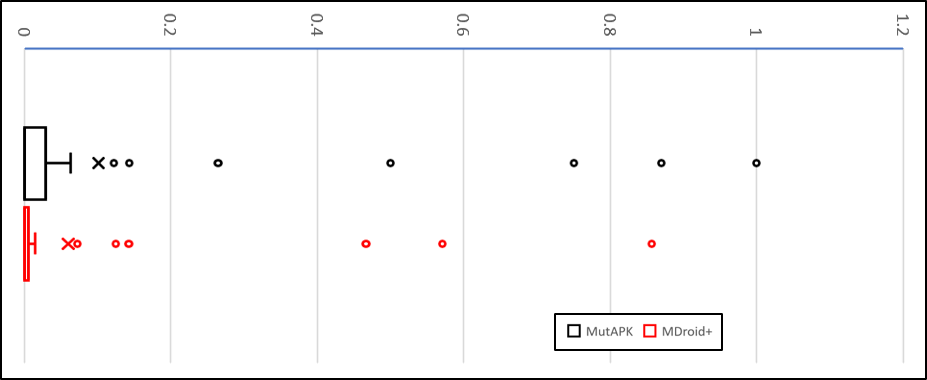
\includegraphics[width=0.35\textheight]{Figures/S22PercNonCompMutMOBP}}
	\caption{Data comparision of MutAPK and MDroid+}
\end{figure}
\end{landscape}

\section{Analysis of non-compilable mutants}

In order to understand the reasons for non-compilable mutants, we analyzed 3 mutants for each one of the mutant operators that generated non-compilable. It is worth noting that this process must be iterative and after finding and fixing the errors, the mutation process must be executed again.

\subsection{31 - InvalidIDFindView}

This operator generated more non-compilable mutants than others. For this operator we found there is an implementation error when the mutation was performed. The correct implementation should be to include \textit{const <constVarName>, 0x<randomlyGeneratedHexa>} before the view was created to assign a random generated value to the key used as view ID. However, we injected \textit{const/16 <constVarName>, 0x<randomlyGeneratedHexa>} that generated a packaging error due to specific instructions that must accompanying \textit{const/16} and not \textit{const}.

After this error was fixed the percentage of non-compilable mutants at app level without taking into account non-shared operators decreases to 4\%.

\subsection{27 - FindViewByIdReturnsNull}

This operator presents two cases we did not consider. Listing \ref{lst:fvbirn1} presents the SMALI representation for finding an Android view; the mutation rule asks to convert the result of the search into a null object. Therefore, Listing \ref{lst:fvbirn2} presents the  SMALI instruction that must be injected instead of the previous one to assign a null value to the result. Nevertheless, after the mutation is performed when the compilation process is launched, an error is displayed on the console (Listing \ref{lst:fvbirn3}), saying that all available registers are between 0 and 15. After a deeper analysis, we found that registers after 16 inclusive are used only for referencing values and a null value could not be assigned. Therefore, we found that a cumbersome process most be made and a verification of the value of the 16th available register must be performed to save the value while the result of the mutation is used, and then the original value can be reassigned to the used register.

This behavior was found in several mutants.

\begin{minipage}{\textwidth}
	\begin{lstlisting}[language={sh}, label={lst:fvbirn1}, caption={SMALI representation of findByViewID method call}, numbers=none]
invoke-virtual {v0, v2}, La2dp/Vol/main;->findViewById(I)Landroid/view/View;

move-result-object v21

check-cast v21, Landroid/widget/Button;
	\end{lstlisting}
\end{minipage}\\

\begin{minipage}{\textwidth}
	\begin{lstlisting}[language={sh}, label={lst:fvbirn2}, caption={SMALI representation of a null value being assigned}, numbers=none]
const/4 v21, 0x0
	\end{lstlisting}
\end{minipage}\\

\begin{minipage}{\textwidth}
	\begin{lstlisting}[language={sh}, label={lst:fvbirn3}, caption={APKTool console response}, numbers=none]
I: Using Apktool 2.3.2
I: Checking whether sources has changed...
I: Smaling smali folder into classes.dex...
test\smali\a2dp\Vol\main.smali[4027,4] Invalid register: v21. Must be between v0 and v15, inclusive.
Could not smali file: a2dp/Vol/main.smali
	\end{lstlisting}
\end{minipage}\\

We found that last line of Listing \ref{lst:fvbirn1} that is in charge of checking the type of the result, is not necessary and can be removed in some cases as it can be seen in Listing \ref{lst:fvbirn4} . Therefore, our implementation search for that instruction to recognize the complete set of instructions that will be replaced. Therefore, MutAPK throws an error when trying to match this expression with next line.

\begin{minipage}{\textwidth}
	\begin{lstlisting}[language={sh}, label={lst:fvbirn4}, caption={APKTool console response}, numbers=none]
invoke-virtual {v7, v9}, Lcom/angrydoughnuts/android/alarmclock/ActivityAlarmNotification;->
	findViewById(I)Landroid/view/View;
	
move-result-object v7
	
invoke-virtual {v7, v12}, Landroid/view/View;->setVisibility(I)V
	\end{lstlisting}
\end{minipage}\\

\subsection{4 - InvalidKeyIntentPutExtra}

Listing \ref{lst:ikipe} shows the result of executing the compilation process over half of the mutants from this mutation operator that are non-compilable. As it can be seen in the listing, the process ends succesfully but no apk file is generated. At this point we think that we might be facing an error within APKTool (\textit{i.e., the tool used for assembling/disassembling an APK}).

\begin{minipage}{\textwidth}
	\begin{lstlisting}[language={sh}, label={lst:ikipe}, caption={Example Output of MutAPK for PhotoStream app}, numbers=none]
I: Using Apktool 2.3.2
I: Checking whether sources has changed...
I: Smaling smali folder into classes.dex...
I: Checking whether resources has changed...
I: Building resources...
S: WARNING: Could not write to (C:\Users\Camilo\AppData\Local\apktool\framework), using C:\Users\Camilo\AppData\Local\Temp\ instead...
S: Please be aware this is a volatile directory and frameworks could go missing, please utilize --frame-path if the default storage directory is unavailable
I: Building apk file...
I: Copying unknown files/dir...
I: Built apk...
	\end{lstlisting}
\end{minipage}\\

If these 4 mutant operators are updated and they do not generate non-compilable mutants, the percentage of non-compilable mutants at APK level (without taking into account the non-shared operators) should be dropped to 0.1\%.





